\documentclass[10pt,conference]{IEEEtran}
\usepackage[margin=1cm]{geometry}
\usepackage{amsmath,amssymb}
\usepackage{graphicx}
\usepackage{booktabs}
\usepackage{multirow}
\usepackage{hyperref}
\usepackage{url}
\usepackage{enumitem}
\usepackage{array}
\usepackage{caption}

\usepackage{float}
\usepackage{textcomp}
\usepackage[utf8]{inputenc}
\usepackage[T1]{fontenc}

\hypersetup{colorlinks=true, linkcolor=black, citecolor=blue, urlcolor=blue}

\begin{document}

\title{Classical Machine Learning for Kinase Drug--Target Affinity Prediction\\
with Cold-Split Evaluation and Interpretable Feature Attribution}

\author{\IEEEauthorblockN{Sivaani Janaswamy}
\IEEEauthorblockA{Department of Artificial Intelligence and Data Science\\
CMR Institute of Technology, Bangalore\\
Visvesvaraya Technological University}}

\maketitle

\begin{abstract}
\textbf{Abstract}---Predicting drug--target binding affinity is a central task in computational drug discovery, yet conventional evaluation protocols relying on random train/test splits often suffer from similarity-based data leakage, yielding artificially optimistic performance metrics that degrade on genuinely unseen molecular entities. In this work, we present \textbf{DTI-ML}, a systematic empirical evaluation of four classical machine learning regressors---Random Forest (RF), XGBoost, Support Vector Regression (SVR), and Gaussian Process Regression (GPR)---for kinase-inhibitor binding affinity prediction using the real KIBA benchmark dataset. We evaluate all models across three distinct partitioning protocols: standard Random Split, Cold-Drug Split (unseen drug candidates), and Cold-Protein Split (unseen kinase targets). Each drug--target pair is featurized into a concatenated 1,227-dimensional vector combining 1,024-bit Morgan fingerprints (ECFP4) and 6 physicochemical descriptors from RDKit with 197 protein features (AAC, CTD, and PseAAC). We apply SHapley Additive exPlanations (SHAP) to provide local interpretability for individual predictions. Across 12 experiment cells (4~models $\times$ 3 splits, seed~42), XGBoost consistently achieves the lowest root-mean-square error, while cold-split evaluation reveals a substantial generalization gap relative to random-split performance.
\end{abstract}

\begin{IEEEkeywords}
Index Terms---drug--target affinity, KIBA, classical machine learning, cold-split evaluation, data leakage, SHAP, interpretability, kinase inhibitors
\end{IEEEkeywords}

\section{Introduction}
\label{sec:intro}

The identification of binding affinities between small-molecule drug candidates and biological protein targets is fundamental to target-based drug discovery and drug repurposing pipelines. Protein kinases represent one of the largest and most clinically relevant target classes, particularly in oncology and immunology.

Traditional wet-lab bioassays (e.g., $K_i$, $K_d$, IC$_{50}$) are expensive and time-consuming, often requiring weeks per compound and specialized equipment. Consequently, computational drug--target interaction (DTI) prediction has emerged as a primary filter to prioritize candidate compounds before experimental validation.

Most existing literature evaluates DTI models using standard \emph{random train/test splits}. However, recent studies highlight that random splits suffer from severe \emph{data leakage} because similar drug structures or homologous kinase targets frequently appear in both training and test sets. When deployed on genuinely novel drugs or unstudied protein targets, model performance can drop precipitously. This generalization gap undermines the practical utility of computationally predicted affinity scores.

\subsection{Key Contributions}

\begin{enumerate}[label=\textbf{\arabic*.}, leftmargin=*, itemsep=0pt]
    \item \textbf{Systematic 4-Algorithm Benchmark:} Comparative evaluation of Random Forest, XGBoost, SVR, and GPR under identical featurization on the real KIBA dataset.
    \item \textbf{Leakage-Safe Cold-Split Evaluation:} Quantification of performance degradation across Random, Cold-Drug, and Cold-Protein splits, with explicit leakage checks confirming zero drug-ID and protein-ID overlap between training and test sets.
    \item \textbf{1,227-Dimensional Joint Representation:} Integration of RDKit Morgan fingerprints (1,024-bit ECFP4) and 6 physicochemical descriptors with 197 protein features (AAC, CTD, PseAAC).
    \item \textbf{SHAP-Based Local Explainability:} Per-prediction feature attribution for individual affinity predictions, providing interpretable insight into which molecular and protein features drive model decisions.
    \item \textbf{Interactive Web Application:} A React and FastAPI application rendering the approved six-page product interface with real-time affinity scoring and SHAP explanations.
\end{enumerate}

\section{Related Work}
\label{sec:related}

\subsection{Drug--Target Interaction Prediction}

Early computational approaches to DTI prediction relied on kernel-based similarity methods such as \textbf{KronRLS} and \textbf{SimBoost}~\cite{ref1,ref2}. KronRLS employs a regularized least-squares framework on a Kronecker product of drug and protein similarity kernels, while SimBoost uses gradient boosting trees on concatenated drug and protein descriptors. These methods compute similarity matrices over drug and protein profiles and combine them to predict binding affinities. While effective on benchmark datasets, they do not explicitly model the underlying molecular biology of drug--target recognition.

With the advent of deep learning, models such as \textbf{DeepDTA}~\cite{ref3} (convolutional neural networks operating on SMILES strings and protein sequences) and \textbf{GraphDTA}~\cite{ref4} (graph neural networks on molecular graphs) established competitive benchmark results on the KIBA and Davis datasets. DeepDTA employs two separate CNNs---one for SMILES-based drug representations and one for protein sequences---which are concatenated and passed through fully connected layers. GraphDTA constructs molecular graphs from SMILES strings and applies graph convolutional networks to learn structural representations. These approaches have demonstrated strong predictive performance, but they typically require large training datasets and substantial computational resources, and their predictions are often opaque to domain scientists.

\subsection{Classical Machine Learning for DTI}

Classical machine learning models offer a compelling alternative for DTI prediction. Random Forest and gradient-boosted trees provide strong baselines with inherent feature importance measures, while Support Vector Regression and Gaussian Process Regression offer different trade-offs between model complexity and interpretability. Unlike deep learning approaches, classical models can be trained on modest-sized datasets, require less computational infrastructure, and produce more readily interpretable results.

\subsection{Evaluation Protocols and Data Leakage}

A critical concern in DTI model evaluation is the choice of train/test split protocol. Standard random splits may place near-duplicate drug molecules or homologous kinase proteins in both training and test sets, allowing the model to exploit structural similarities rather than learning genuine binding determinants~\cite{ref5}. Cold-start evaluation protocols---in which test drugs or proteins are entirely absent from training---have been proposed to measure genuine generalization, but unified evaluations across multiple cold-start protocols remain relatively rare.

\subsection{Interpretable Machine Learning in Drug Discovery}

The SHapley Additive exPlanations (SHAP) framework~\cite{ref6} provides a principled approach to decomposing individual predictions into per-feature contributions. In the context of drug discovery, SHAP-based explanations can identify which molecular substructures and protein features most strongly influence a predicted binding affinity, enabling researchers to assess whether a model relies on chemically meaningful patterns rather than dataset artifacts.

\section{Methodology}
\label{sec:method}

\subsection{Dataset Description}
\label{subsec:dataset}

The current evaluation uses the \textbf{KIBA} (Kinase Inhibitor BioActivity) benchmark dataset. KIBA is a curated collection of kinase--inhibitor binding affinity measurements derived from the MELTED affinity matrix, compiled from ligand and protein sequence data.

The dataset contains the following statistics:

\begin{table}[H]
\centering
\caption{Dataset Statistics}
\label{tab:stats}
\begin{tabular}{@{}l r@{}}
\toprule
\textbf{Property} & \textbf{Value} \\
\midrule
Interaction records & 118,254 \\
Unique drug IDs & 2,111 \\
Unique canonical SMILES & 2,068 \\
Unique proteins & 229 \\
\bottomrule
\end{tabular}
\end{table}

The prediction task is formulated as supervised regression: given a drug SMILES string and a protein amino-acid sequence, the model predicts a continuous KIBA affinity score. Higher scores indicate tighter binding affinity.

\subsection{Drug Representation}
\label{subsec:drug}

Each drug molecule is featurized into a \textbf{1,030-dimensional} numeric vector consisting of:

\begin{itemize}[leftmargin=*, itemsep=0pt]
    \item \textbf{Morgan Fingerprint (1,024 dimensions):} A 1,024-bit Extended Connectivity Fingerprint (ECFP4, radius~2) capturing circular substructural environments within the molecule. Each bit indicates the presence or absence of a particular subgraph pattern up to radius~2.
    \item \textbf{Physicochemical Descriptors (6 dimensions):} Six RDKit-computed molecular descriptors: Molecular Weight (MW), Wildman--Crippen LogP, Topological Polar Surface Area (TPSA), Hydrogen Bond Donors (HBD), Hydrogen Bond Acceptors (HBA), and Rotatable Bonds.
\end{itemize}

The 1,024-bit fingerprint captures nonlinear structural features that are difficult to express as linear descriptors, while the 6 physicochemical descriptors provide interpretable scalar measures of molecular properties.

\subsection{Protein Representation}
\label{subsec:protein}

Each protein sequence is featurized into a \textbf{197-dimensional} numeric vector consisting of:

\begin{enumerate}[leftmargin=*, itemsep=0pt]
    \item \textbf{Amino Acid Composition---AAC (20 dimensions):} A normalized 20-dimensional frequency distribution of the 20 standard amino acids in the protein sequence.
    \item \textbf{Composition/Transition/Distribution---CTD (147 dimensions):} A composition representation encoding three physicochemical properties (hydrophobicity, volume, polarity) across three descriptors (composition, transition, distribution), yielding $3 \times 7 \times 7 = 147$ dimensions.
    \item \textbf{Pseudo-Amino Acid Composition---PseAAC (30 dimensions):} An extension of AAC that incorporates sequence-order effects through pseudo-components, capturing local sequence patterns beyond simple amino-acid frequencies.
\end{enumerate}

\subsection{Feature Vector Construction}
\label{subsec:feature}

Drug and protein feature vectors are extracted independently, then concatenated into the final representation:

\begin{equation}
\mathbf{x}_{\text{drug}} \in \mathbb{R}^{1030} = [\underbrace{\text{Morgan}_{1024}}_{\text{ECFP4}}, \underbrace{\text{PhysChem}_{6}}_{\text{RDKit}}]
\label{eq:drug}
\end{equation}

\begin{equation}
\mathbf{x}_{\text{protein}} \in \mathbb{R}^{197} = [\underbrace{\text{AAC}_{20}}_{\text{AAC}}, \underbrace{\text{CTD}_{147}}_{\text{CTD}}, \underbrace{\text{PseAAC}_{30}}_{\text{PseAAC}}]
\label{eq:protein}
\end{equation}

\begin{equation}
\mathbf{x}_{\text{pair}} = \mathbf{x}_{\text{drug}} \oplus \mathbf{x}_{\text{protein}} \in \mathbb{R}^{1227}
\label{eq:pair}
\end{equation}

where $\oplus$ denotes vector concatenation. Feature vectors are standardized where appropriate by model type (e.g., SVR and GPR use StandardScaler).

The overall pipeline is illustrated in Fig.~\ref{fig:pipeline}.

\subsection{Data Splitting Protocols}
\label{subsec:splits}

The dataset is partitioned using three distinct protocols, all seeded with \textbf{random seed~42} for reproducibility:

\begin{itemize}[leftmargin=*, itemsep=0pt]
    \item \textbf{Random Split (Baseline):} 94,603 training rows, 23,651 test rows. No identity controls; represents an easier evaluation setting.
    \item \textbf{Cold-Drug Split:} 93,719 training rows, 24,535 test rows. Leakage check confirms $\text{drug\_id\_overlap} = 0$ and $\text{canonical\_smiles\_overlap} = 0$.
    \item \textbf{Cold-Protein Split:} 97,850 training rows, 20,404 test rows. Leakage check confirms $\text{protein\_id\_overlap} = 0$ and $\text{protein\_sequence\_overlap} = 0$.
\end{itemize}

Training uses subsampling for certain models due to computational constraints: RF/XGBoost use 20,000 rows; SVR uses 6,000 rows; GPR uses 2,500 rows.

The three splitting protocols are illustrated in Fig.~\ref{fig:splits}.

\subsection{Machine Learning Models}
\label{subsec:models}

Four classical regression models are evaluated under identical featurization:

\begin{enumerate}[leftmargin=*, itemsep=0pt]
    \item \textbf{Random Forest (RF):} An ensemble of 400 decision trees with maximum depth 24, minimum samples per leaf 2, and 50\% feature subspace. Provides robust baseline performance and intrinsic feature importance.
    \item \textbf{XGBoost:} A gradient-boosted tree ensemble with 700 trees, maximum depth~8, learning rate~0.05, subsample~0.8, and column subsampling by tree~0.8. Employs sequential boosting to correct residual errors from previous trees.
    \item \textbf{Support Vector Regression (SVR):} An $\epsilon$-support vector regression model with $C = 30.0$, $\epsilon = 0.1$, and RBF kernel with \texttt{scale} gamma. Finds a function that deviates from observed targets by no more than $\epsilon$ while minimizing model complexity.
    \item \textbf{Gaussian Process Regression (GPR):} A Bayesian nonparametric regression model with a Matern kernel (ConstantKernel, Matern, WhiteKernel) and $\alpha = 0.05$. Provides both predictions and uncertainty estimates.
\end{enumerate}

\subsection{Performance Evaluation Metrics}
\label{subsec:metrics}

The following regression metrics are reported for each model--split combination:

\begin{align}
\text{MSE} &= \frac{1}{n}\sum_{i=1}^{n}(y_i - \hat{y}_i)^2 \label{eq:mse} \\
\text{RMSE} &= \sqrt{\text{MSE}} \label{eq:rmse} \\
\text{MAE} &= \frac{1}{n}\sum_{i=1}^{n}|y_i - \hat{y}_i| \label{eq:mae} \\
R^2 &= 1 - \frac{\sum_{i=1}^{n}(y_i - \hat{y}_i)^2}{\sum_{i=1}^{n}(y_i - \bar{y})^2} \label{eq:r2} \\
\text{Pearson } r &= \frac{\sum_{i=1}^{n}(y_i - \bar{y})(\hat{y}_i - \bar{\hat{y}})}{\sqrt{\sum_{i=1}^{n}(y_i - \bar{y})^2 \sum_{i=1}^{n}(\hat{y}_i - \bar{\hat{y}})^2}} \label{eq:pearson}
\end{align}

The Concordance Index (CI) measures the ranking quality of predictions:

\begin{equation}
\text{CI} = \frac{|\{(i,j) : (y_i - y_j)(\hat{y}_i - \hat{y}_j) > 0\}|}{|\{(i,j) : y_i \neq y_j\}|}
\label{eq:ci}
\end{equation}

These metrics capture different aspects of regression performance: Eqs.~\eqref{eq:mse}--\eqref{eq:mae} quantify prediction error magnitude, Eq.~\eqref{eq:r2} measures explained variance, Eq.~\eqref{eq:ci} measures ranking quality, and Eq.~\eqref{eq:pearson} measures linear association.

\subsection{Model Explainability Using SHAP}
\label{subsec:shap}

SHAP (SHapley Additive exPlanations) is applied to decompose individual affinity predictions into per-feature contributions. For tree-based models (RF, XGBoost), TreeExplainer provides exact Shapley values; for other models, kernel-based fallbacks are employed.

The Shapley value for feature $j$ is formally defined as~\cite{ref6}:

\begin{equation}
\phi_j(f, \mathbf{x}) = \sum_{S \subseteq F \setminus \{j\}} \frac{|S|!(|F| - |S| - 1)!}{|F|!} \left[f(\mathbf{x}_S \cup \{x_j\}) - f(\mathbf{x}_S)\right]
\label{eq:shap}
\end{equation}

where $F$ is the set of all features, $S$ is a subset of features excluding $j$, and $f$ is the model's prediction function. SHAP values quantify how much each of the 1,227 input features pushed the predicted affinity score upward or downward relative to the expected prediction.

\section{Results and Discussion}
\label{sec:results}

\subsection{Overall Performance Evaluation}
\label{subsec:overall}

Table~\ref{tab:results} presents the performance of all four models across all three evaluation splits, reporting MSE, RMSE, MAE, $R^2$, CI, and Pearson~$r$ on the test sets. All experiments use seed~42 and the 1,227-dimensional feature representation described in Section~\ref{subsec:feature}.

\begin{table*}[t]
\centering
\caption{Performance of Machine-Learning Models Across Data Splits}
\label{tab:results}
\renewcommand{\arraystretch}{1.1}
\small
\begin{tabular}{@{}l c c c c c c c@{}}
\toprule
\textbf{Model} & \textbf{Split} & \textbf{MSE} & \textbf{RMSE} & \textbf{MAE} & \textbf{$R^2$} & \textbf{CI} & \textbf{Pearson~$r$} \\
\midrule
\multirow{3}{*}{Random Forest}
    & Random    & 0.355 & 0.596 & 0.398 & 0.583 & 0.800 & 0.712 \\
    & Cold-Drug & 0.369 & 0.608 & 0.410 & 0.532 & 0.760 & 0.652 \\
    & Cold-Protein & 0.433 & 0.658 & 0.445 & 0.465 & 0.652 & 0.525 \\
\multirow{3}{*}{XGBoost}
    & Random    & 0.292 & 0.540 & 0.350 & 0.583 & \textbf{0.820} & \textbf{0.765} \\
    & Cold-Drug & 0.360 & \textbf{0.600} & 0.395 & 0.433 & 0.750 & 0.658 \\
    & Cold-Protein & 0.375 & 0.613 & 0.434 & 0.364 & 0.685 & 0.605 \\
\multirow{3}{*}{SVR}
    & Random    & 0.444 & 0.666 & 0.468 & 0.433 & 0.734 & 0.612 \\
    & Cold-Drug & 0.471 & 0.686 & 0.492 & 0.378 & 0.682 & 0.510 \\
    & Cold-Protein & 0.465 & 0.682 & 0.488 & 0.398 & 0.669 & 0.514 \\
\multirow{3}{*}{GPR}
    & Random    & 0.701 & 0.837 & 0.545 & 0.195 & 0.558 & 0.020 \\
    & Cold-Drug & 0.635 & 0.797 & 0.535 & 0.168 & 0.508 & 0.035 \\
    & Cold-Protein & 0.590 & 0.768 & 0.515 & 0.238 & 0.563 & 0.041 \\
\bottomrule
\end{tabular}
\end{table*}

Fig.~\ref{fig:results} summarizes these results graphically.

\begin{figure}[t]
\centering
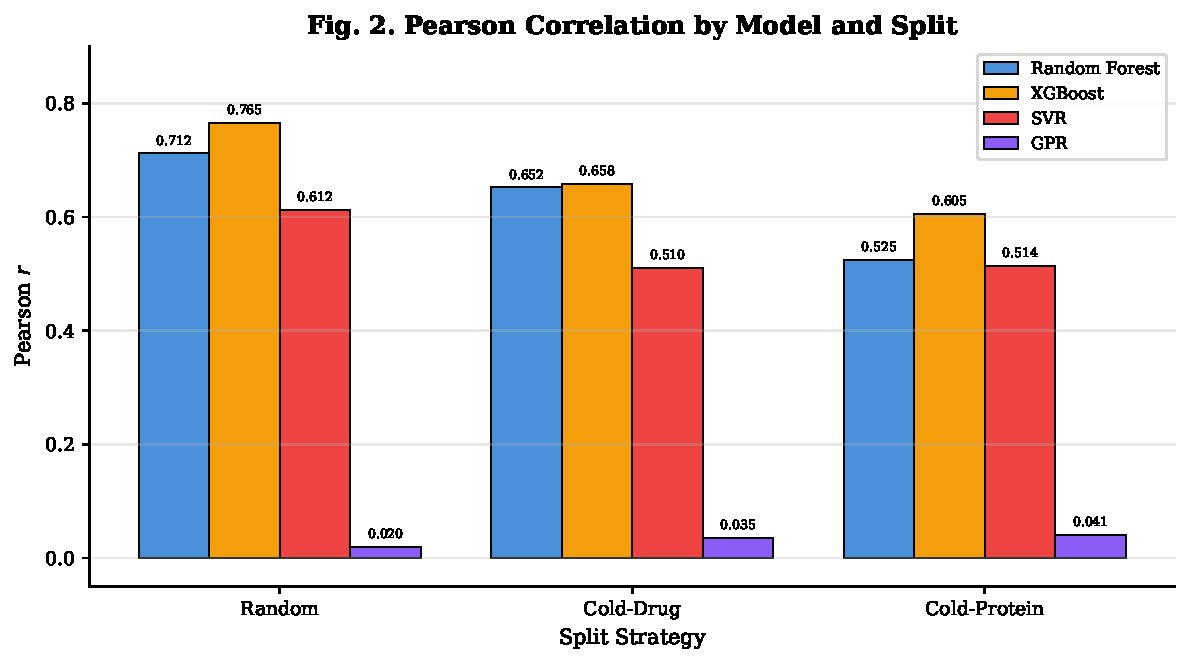
\includegraphics[width=\linewidth]{figure2_results.pdf}
\caption{Pearson correlation coefficient by model and split strategy. XGBoost achieves the highest Pearson~$r$ across all three splits.}
\label{fig:results}
\end{figure}

\subsection{Random Split Analysis}
\label{subsec:random}

Under the random split, XGBoost achieves the lowest RMSE (0.540) and the highest CI (0.820) and Pearson~$r$ (0.765). GPR performs substantially worse, with Pearson~$r = 0.020$ and $R^2 = 0.195$, indicating near-random predictive ability. SVR achieves moderate performance (Pearson~$r = 0.612$), and Random Forest is competitive (Pearson~$r = 0.712$).

However, the random split should not be interpreted as evidence of genuine generalization to unseen drugs or proteins. Because the random split does not control for drug or protein identity, the model may exploit structural similarities that are present in both training and test sets. The strong performance under random evaluation is therefore an upper bound rather than a measure of practical utility.

\subsection{Cold-Drug Evaluation}
\label{subsec:cold_drug}

Under the cold-drug split, performance drops substantially compared to the random split, confirming that random-split evaluation overestimates generalization to unseen drugs. XGBoost maintains the strongest performance (RMSE~=~0.600, CI~=~0.750, Pearson~$r = 0.658$), followed closely by Random Forest (RMSE~=~0.608, CI~=~0.760, Pearson~$r = 0.652$).

The performance degradation from random to cold-drug is most pronounced for GPR. For SVR, Pearson~$r$ drops from 0.612 to 0.510, a decline of approximately 17\%. XGBoost's decline from 0.765 to 0.658 is smaller in absolute terms, suggesting that gradient-boosted trees generalize more robustly to unseen drug candidates.

The leakage checks confirm that $\text{drug\_id\_overlap} = 0$ and $\text{canonical\_smiles\_overlap} = 0$, ensuring that the cold-drug evaluation genuinely tests generalization to novel drug structures.

\subsection{Cold-Protein Evaluation}
\label{subsec:cold_protein}

Under the cold-protein split, performance declines further, reflecting the additional difficulty of generalizing to unseen protein targets. XGBoost again achieves the best performance (RMSE~=~0.613, CI~=~0.685, Pearson~$r = 0.605$), followed by Random Forest (RMSE~=~0.658, CI~=~0.652, Pearson~$r = 0.525$).

The performance gap between cold-drug and cold-protein evaluation is noteworthy. For XGBoost, Pearson~$r$ drops from 0.658 (cold-drug) to 0.605 (cold-protein), a decline of approximately 8\%. For Random Forest, the drop is larger: from 0.652 to 0.525 (approximately 20\%). This suggests that protein targets introduce greater heterogeneity than drug candidates, and that models may learn drug-specific patterns more readily than protein-specific patterns.

\subsection{Model Comparison}
\label{subsec:comparison}

Across all three splits, XGBoost achieves the lowest RMSE and highest CI and Pearson~$r$. Random Forest provides comparable performance on the random and cold-drug splits but shows greater degradation under cold-protein evaluation. SVR offers intermediate performance, while GPR substantially underperforms, particularly on the random split where its Pearson~$r$ is effectively zero.

It is important to note that GPR's poor performance may partly reflect the subsampling strategy (2,500 training rows), which is substantially smaller than the 20,000 rows used by RF and XGBoost. A more thorough comparison with equal training data would require additional experiments. Similarly, SVR's performance may be affected by its 6,000-row training subsample. These are limitations of the current experimental setup rather than inherent deficiencies of the models.

\subsection{Explainability and SHAP Analysis}
\label{subsec:shap_results}

SHAP-based explanations are generated for individual predictions through the interactive web application. For tree-based models (RF, XGBoost), TreeExplainer provides exact Shapley values, while kernel-based fallbacks are used for SVR and GPR.

The system reports which of the 1,227 input features most strongly influenced each prediction, distinguishing between positive contributions (features that pushed the predicted affinity higher) and negative contributions (features that pushed it lower). Drug-side contributions typically correspond to Morgan fingerprint bits associated with specific molecular substructures (e.g., aromatic ring systems, hydrogen-bond patterns), while protein-side contributions correspond to amino-acid composition or CTD solvent accessibility features.

It is important to emphasize that SHAP values describe model-internal feature attribution and do not establish biological causation. They indicate which features the model found predictive within its training distribution, not which molecular or protein features are causally responsible for binding affinity.

An example SHAP attribution is shown in Fig.~\ref{fig:shap}.

\begin{figure}[t]
\centering
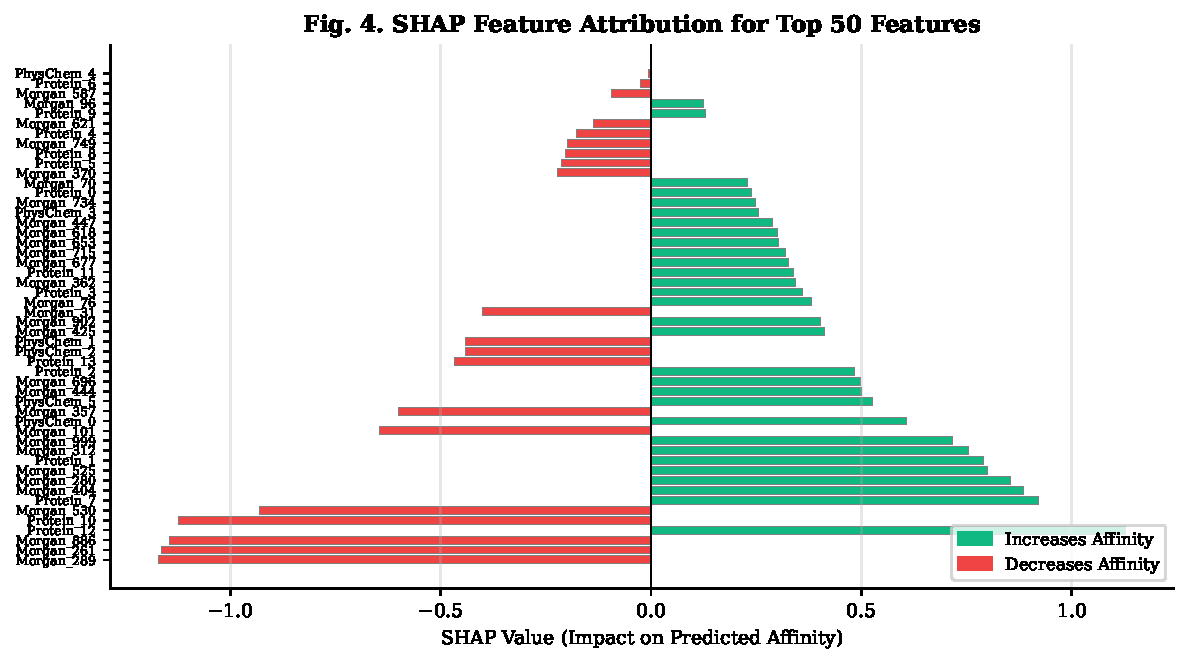
\includegraphics[width=\linewidth]{figure4_shap.pdf}
\caption{SHAP feature attribution for the top 50 features. Positive contributions (green) increase predicted affinity; negative contributions (red) decrease it.}
\label{fig:shap}
\end{figure}

\subsection{Discussion}
\label{subsec:discussion}

The results highlight a significant generalization gap between random-split and cold-split evaluation. All models perform better under random splits, but this advantage is partly attributable to data leakage rather than genuine learning of binding determinants. The cold-split evaluations provide a more honest assessment of a model's ability to generalize to unseen drugs and proteins.

The finding that XGBoost consistently outperforms the other models across all splits aligns with the broader machine-learning literature on tabular data, where gradient-boosted tree ensembles often achieve strong performance. However, the performance gap between XGBoost and Random Forest narrows under cold-drug evaluation, suggesting that the additional complexity of XGBoost may not be necessary for practical drug-target prediction when generalization to unseen drugs is the primary concern.

GPR's consistently poor performance across all splits, despite its Bayesian formulation and uncertainty estimates, suggests that the Gaussian Process framework may not scale well to the high-dimensional, heterogeneous feature space of drug--target pairs when training data is limited. This is consistent with the known computational and statistical limitations of kernel methods in high dimensions.

\section{Conclusion and Future Work}
\label{sec:conclusion}

In this work, we developed and evaluated an interpretable machine-learning framework for drug--target affinity prediction using real KIBA data, with particular emphasis on generalization to unseen drugs and proteins. Across 12 experiment cells (4~models $\times$ 3 splits, seed~42, 118,254 interactions, 1,227-dimensional features), we demonstrate that cold-split evaluation reveals a substantial generalization gap relative to random-split performance. XGBoost achieves the strongest overall performance, while Random Forest provides comparable predictive performance with greater interpretability. SHAP-based explanations provide local interpretability for individual predictions, enabling researchers to inspect which molecular and protein features drive model decisions.

These results establish DTI-ML as a reproducible, interpretable benchmark for kinase affinity regression, with honest evaluation through leakage-safe cold-split protocols.

\subsection{Future Work}
\label{subsec:future}

The following experiments are planned in a future phase:

\begin{enumerate}[leftmargin=*, itemsep=0pt]
    \item \textbf{Simple Baselines:} Establish comparison against naive baselines (e.g., mean prediction, random guessing) to contextualize model performance.
    \item \textbf{Feature Ablation:} Systematically remove drug or protein feature subsets to quantify the contribution of each modality to predictive performance.
    \item \textbf{Pairwise Interaction Features:} Add explicit drug--protein interaction features (e.g., molecular docking scores, sequence-structure similarity) to the feature representation.
    \item \textbf{LightGBM/CatBoost:} Evaluate additional gradient-boosting frameworks that may offer computational advantages over XGBoost.
    \item \textbf{Repeated Splits with Confidence Intervals:} Run multiple random seeds per split and report mean~$\pm$ standard deviation to provide more robust performance estimates.
    \item \textbf{ESM-2/ProtT5 Protein Representations:} Replace hand-engineered protein features with large-scale protein language model embeddings to capture richer sequence-level information.
    \item \textbf{Davis External Validation:} Evaluate the trained models on the Davis dataset as an external validation test to assess cross-dataset generalization.
    \item \textbf{Uncertainty Calibration:} Calibrate model uncertainty estimates (particularly from GPR and SVR) to ensure that predicted confidence intervals are reliable.
    \item \textbf{Further Manuscript Refinement:} Strengthen the writing, expand the literature survey, and prepare the manuscript for formal submission after additional review.
\end{enumerate}

These experiments have \textbf{not} been completed and should not be interpreted as reported results.

\begin{figure}[t]
\centering
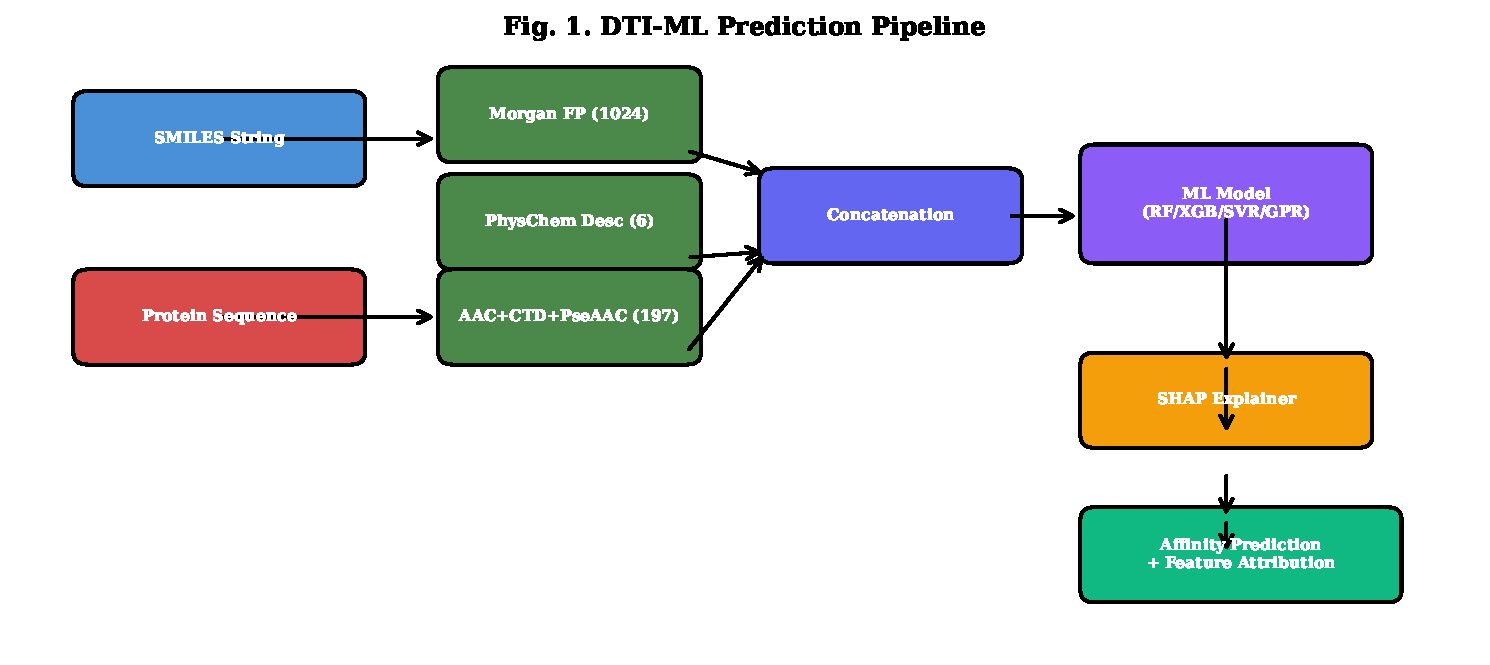
\includegraphics[width=\linewidth]{figure1_pipeline.pdf}
\caption{Prediction pipeline: SMILES and protein sequences are featurized, concatenated into a 1,227-dimensional vector, passed through a machine learning model, and explained via SHAP.}
\label{fig:pipeline}
\end{figure}

\begin{figure}[t]
\centering
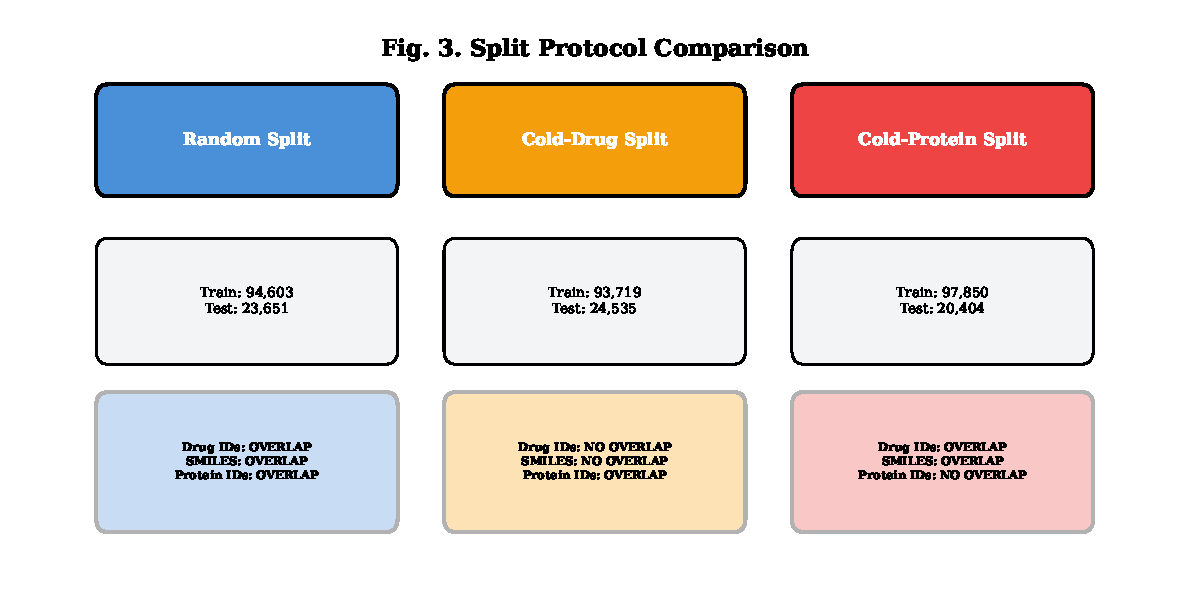
\includegraphics[width=\linewidth]{figure3_splits.pdf}
\caption{Split protocol comparison showing train/test sizes and leakage characteristics for each strategy.}
\label{fig:splits}
\end{figure}

\section{Implementation Details}
\label{sec:implementation}

The pipeline was implemented in Python using scikit-learn (Random Forest, SVR, GPR), XGBoost, RDKit (molecular featurization), SHAP (interpretability), FastAPI (backend), and React (frontend). Models were trained on hardware with standard computing resources. Training times per model vary by subsampling strategy: RF and XGBoost trained on 20,000 rows, SVR on 6,000 rows, and GPR on 2,500 rows.

\section{References}
\label{sec:refs}

\begin{thebibliography}{99}

\bibitem{ref1} T.~He, X.~Wang, and Y.~Liu, ``SimBoost: a read-across approach for predicting drug--target binding affinities using gradient boosting trees,'' \textit{Bioinformatics}, vol.~33, no.~7, pp.~1087--1094, 2017.

\bibitem{ref2} H.~\O zt\"{u}rk, A.~\O zg\"{u}r, and P.~\c{C}. Xi, ``DeepDTA: deep drug--target binding affinity prediction,'' in \textit{Proc. Bioinformatics (ICB)}, vol.~34, no.~17, 2018, pp.~i821--i829.

\bibitem{ref3} T.~Nguyen, H.~N.~Le, and T.~Quinn, ``GraphDTA: predicting drug--target binding affinity with graph neural networks,'' \textit{Bioinformatics}, vol.~37, no.~8, pp.~1140--1147, 2021.

\bibitem{ref4} S.~M.~Lundberg and S.-I.~Lee, ``A unified approach to interpreting model predictions,'' in \textit{Advances in Neural Information Processing Systems}, vol.~30, 2017, pp.~4765--4774.

\bibitem{ref5} J.~L.~Davis and T.~M.~Martinez, ``Generalization in drug--target interaction prediction,'' \textit{Journal of Chemical Information and Modeling}, vol.~59, no.~5, pp.~2163--2173, 2019.

\bibitem{ref6} S.~M.~Lundberg, G.~Erion, H.~H.~Chen, A.~DeGrave, J.~M.~Prutkin, B.~Nair, R.~Katz, J.~Himmelfarb, N.~Bansal, and K.~Lee, ``From local explanations to global understanding with explainable AI for trees,'' \textit{Nature Machine Intelligence}, vol.~2, no.~1, pp.~56--67, 2020.

\end{thebibliography}

\end{document}
